\documentclass[11pt,a4paper]{article}

% ── Packages ────────────────────────────────────────────────────────────────
\usepackage[margin=1in]{geometry}
\usepackage{amsmath,amssymb,amsthm}
\usepackage{graphicx}
\usepackage{booktabs}
\usepackage{tabularx}
\usepackage{xcolor}
\usepackage{hyperref}
\usepackage{listings}
\usepackage{tikz}
\usepackage{pgfplots}
\pgfplotsset{compat=1.18}
\usetikzlibrary{positioning,arrows.meta,shapes.geometric,fit,backgrounds,calc,matrix,decorations.pathreplacing}
\usepackage{caption}
\usepackage{subcaption}
\usepackage{enumitem}
\usepackage{algorithm}
\usepackage{algpseudocode}
\usepackage{microtype}
\usepackage{fancyhdr}
\usepackage{multirow}

% ── Hyperref styling ────────────────────────────────────────────────────────
\hypersetup{
  colorlinks=true,
  linkcolor=blue!60!black,
  citecolor=blue!60!black,
  urlcolor=teal!70!black,
  pdftitle={Heterogeneous Graph-Attention RL for Indian Equity Portfolio Allocation},
  pdfauthor={Jash},
}

% ── Listings (Python) ───────────────────────────────────────────────────────
\definecolor{codebg}{RGB}{248,248,248}
\definecolor{codekw}{RGB}{20,80,160}
\definecolor{codestr}{RGB}{120,40,40}
\definecolor{codecom}{RGB}{80,120,80}
\lstdefinestyle{py}{
  language=Python,
  backgroundcolor=\color{codebg},
  basicstyle=\ttfamily\footnotesize,
  keywordstyle=\color{codekw}\bfseries,
  stringstyle=\color{codestr},
  commentstyle=\color{codecom}\itshape,
  numbers=left, numberstyle=\tiny\color{gray},
  numbersep=8pt, stepnumber=1,
  frame=single, framesep=4pt, rulecolor=\color{gray!30},
  showstringspaces=false, breaklines=true,
  tabsize=4,
  literate={─}{{-}}1
}
\lstset{style=py}

% ── Title ───────────────────────────────────────────────────────────────────
\title{
  \vspace{-1cm}
  \Large\textbf{Heterogeneous Graph-Attention Reinforcement Learning for \\
  Indian Equity Portfolio Allocation} \\[0.3em]
  \large A Technical Report on Architecture, Implementation, and the Path to a Working Baseline
}
\author{Trading Bot Project --- Milestones M0 through M6}
\date{April 2026}

% ── Headers ─────────────────────────────────────────────────────────────────
\pagestyle{fancy}
\fancyhf{}
\fancyhead[L]{\small Heterogeneous Graph-Attention RL for Equity Allocation}
\fancyhead[R]{\small \thepage}
\renewcommand{\headrulewidth}{0.4pt}

\begin{document}

\maketitle
\thispagestyle{empty}

% ────────────────────────────────────────────────────────────────────────────
% Abstract
% ────────────────────────────────────────────────────────────────────────────
\begin{abstract}
\noindent We present the design and implementation of a deep reinforcement learning system
for daily portfolio allocation over a 163-stock Indian equity universe (NIFTY 50 augmented with
sectoral leaders). The agent is a heterogeneous graph attention network operating on stock and
sector nodes, fed by a temporal convolutional encoder over a 60-day feature window, and trained
end-to-end with Proximal Policy Optimization (PPO). We document the full pipeline from raw
yfinance bars through walk-forward training, including a Postgres-backed paper-broker
infrastructure stub for downstream evaluation. Beyond architecture, we report on a sequence of
non-trivial bugs discovered during initial training runs --- a \emph{Differential Sharpe} reward
with zero expected value at steady state, raw input features spanning eleven orders of magnitude
in scale, and a Python-loop bottleneck in the environment that disguised itself as a GPU-bound
problem. After fixing each, the simpler intra-sector graph variant achieves the first positive
training Sharpe in the project's history. We close with a roster of pre-staged improvements for
the next training round and a path to walk-forward evaluation.
\end{abstract}

\tableofcontents
\newpage

% ════════════════════════════════════════════════════════════════════════════
\section{Introduction}
% ════════════════════════════════════════════════════════════════════════════

\subsection{Goal}

Build a local, paper-trading-capable reinforcement learning system that learns a daily
portfolio-allocation policy over the Indian equity universe (NSE), using a graph-aware
neural network over intra-sector and inter-sector relationships, trained on roughly ten
years of historical data, with a Postgres-backed simulated broker and stubbed hooks for
live Zerodha Kite trading.

The agent decides, each trading day, what fraction of capital to hold in cash and what
fraction to allocate to each of $N$ tradeable stocks, subject to long-only and per-name
weight cap constraints. Quality is measured by net-of-cost Sharpe ratio against
representative baselines (equal-weight rebalanced, buy-and-hold index, momentum top-K,
60/40 cash, and uniform random).

\subsection{Non-goals (v1)}

\begin{itemize}
\item Real-money live trading (interfaces only; disabled by default).
\item Sub-minute or tick-level data (daily bars; intraday is a future variant).
\item LLM-in-the-loop at inference time (sentiment, if used at all, is offline).
\item Multi-user / multi-account / hardened production deployment.
\end{itemize}

\subsection{Design Principles}

\begin{enumerate}[leftmargin=*]
\item \textbf{Strict temporal separation.} Features at day $t$ use only data with
timestamp $\le t-1$ for actions executed on day $t$. Actions are placed at the open
of day $t$; portfolio is marked-to-close.

\item \textbf{Universe as of date.} Historical universe snapshots prevent
survivorship bias --- selecting ``today's top N per sector'' and backtesting on ten
years is selecting winners after the fact.

\item \textbf{Mask, don't impute.} Stocks not yet listed (or delisted) are masked
out of the observation and action space for the relevant dates. No zero-filling
of non-existent tickers.

\item \textbf{Broker-agnostic.} A \texttt{Broker} ABC with a paper implementation
backed by Postgres, and a Zerodha Kite stub. The live adapter is behind a flag that
is off by default.

\item \textbf{Reproducibility.} Seeds pinned, data snapshotted with a SHA256 hash,
\texttt{uv lock} for dependencies, MLflow for runs, dockerized Postgres.

\item \textbf{Baselines first.} Buy-and-hold NIFTY 50, equal-weight monthly
rebalance, momentum top-K, and 60/40 are implemented and measured \emph{before}
the RL agent. The RL agent has to beat them net of costs.

\item \textbf{One end-to-end path before specialization.} A minimal flat-feature
PPO run must work on the full pipeline before GNN, sentiment, or hierarchical
policies are added.
\end{enumerate}

\subsection{Milestone Roadmap}

\begin{table}[h]
\centering
\caption{Project milestones and current status as of April 26, 2026.}
\begin{tabularx}{\textwidth}{l X l}
\toprule
\textbf{Milestone} & \textbf{Scope} & \textbf{Status} \\
\midrule
M0 & Repo skeleton, \texttt{uv}, ruff, mypy, pytest, dockerized Postgres + MLflow & Complete \\
M1 & Database schema; SQLAlchemy 2.0 models; Alembic migration & Complete \\
M2 & Data ingestion; yfinance source; Kaggle stub; Zerodha stub & Complete \\
M3 & Alignment + features; train/val/test panels with SHA256 sidecars & Complete \\
M4 & \texttt{PanelTradingEnv} + cost model + reward + 5 baselines & Complete \\
M5 & MLP policy + PPO; CleanRL-style single-file trainer & Complete \\
M6 & Heterogeneous GNN with sector hierarchy + 3 ablation configs & Complete \\
M7 & Walk-forward training & Pending \\
M8 & Paper broker; T+1 settlement; ledger reports & Pending \\
M9 & Zerodha adapter stub & Pending \\
M10 & End-to-end report; attention heatmaps; significance tests & Pending \\
\bottomrule
\end{tabularx}
\end{table}

\subsection{Hardware and Software Stack}

Development is performed on macOS (Apple Silicon, MPS backend); training runs are
executed on a Linux server with CUDA 12.8 and an RTX 5090 (Blackwell). Software stack:
Python 3.12, PyTorch (BF16 autocast), \texttt{torch\_geometric} for GAT layers,
Polars for tabular data, NumPy/numba-style numpy-only env code, Hydra for
configuration, MLflow for experiment tracking.

% ════════════════════════════════════════════════════════════════════════════
\section{Data Pipeline}
% ════════════════════════════════════════════════════════════════════════════

\subsection{Universe Construction}

The universe consists of 163 NSE-listed equities organized into 8 sectors of roughly
equal size. The sector taxonomy was constructed manually from sectoral indices and
is fixed across the entire training period. Table~\ref{tab:universe} summarises.

\begin{table}[h]
\centering
\caption{Sector composition of the 163-stock universe. Sector IDs are 1-indexed; ID 0
is reserved for ``unclassified'' (used internally only --- no stock in the universe
falls into this bucket).}
\label{tab:universe}
\small
\begin{tabularx}{\textwidth}{l c X}
\toprule
\textbf{Sector} & \textbf{ID} & \textbf{Representative tickers} \\
\midrule
Banking + NBFC + Insurance & 1 & HDFCBANK, ICICIBANK, KOTAKBANK, BAJFINANCE, SBIN, \ldots \\
Information Technology & 2 & TCS, INFY, HCLTECH, WIPRO, LTIM, MPHASIS, \ldots \\
Pharma + Healthcare & 3 & SUNPHARMA, DRREDDY, CIPLA, DIVISLAB, APOLLOHOSP, \ldots \\
Automotive & 4 & MARUTI, M\&M, BAJAJ-AUTO, EICHERMOT, TATAMOTORS, \ldots \\
Oil, Gas \& Power & 5 & RELIANCE, ONGC, BPCL, NTPC, POWERGRID, COALINDIA, \ldots \\
Metals \& Mining & 6 & TATASTEEL, JSWSTEEL, HINDALCO, COALINDIA, NMDC, \ldots \\
Consumer + Retail & 7 & ITC, HINDUNILVR, NESTLEIND, BRITANNIA, ASIANPAINT, \ldots \\
Capital Goods + Defence + Cement & 8 & LT, SIEMENS, ABB, BHEL, HAL, ULTRACEMCO, \ldots \\
\bottomrule
\end{tabularx}
\end{table}

\subsection{Sources}

Three concrete data sources implement a common \texttt{MarketDataSource} Protocol:

\begin{itemize}[leftmargin=*]
\item \texttt{YFinanceSource} --- primary source; per-ticker cache at\\
\texttt{data/raw/yfinance/<ticker>/<start>\_<end>.parquet} with exponential backoff
and \texttt{auto\_adjust=True} (so close prices are split- and dividend-adjusted).
\item \texttt{KaggleSource} --- backfill source for delisted or pre-IPO tickers,
loaded from \texttt{data/raw/kaggle/<TICKER>.parquet}.
\item \texttt{ZerodhaSource} --- interface stub for live data; raises
\texttt{NotImplementedError}.
\end{itemize}

\subsection{Storage Layout}

OHLCV is partitioned Hive-style at\\
\texttt{data/ohlcv/year=YYYY/ticker=TICKER.parquet} with idempotent writes (rerunning
\texttt{scripts/fetch\_data.py} is a no-op on already-cached date ranges).

\subsection{Alignment and Masking}

\texttt{src/trader/data/alignment.py} produces a dense $(date \times ticker)$ panel
using the NSE trading calendar derived from the union of observed dates across all
tickers. The key invariant:

\begin{quote}
\itshape
A ticker that was first listed in 2017 has \texttt{is\_tradeable = False} for all
dates in 2014--2016. Its rows still exist in the panel, but with \texttt{adj\_close = 0}
sentinel and \texttt{is\_tradeable = False}, so models and the env must consult the
mask to know which stocks are actionable on each date.
\end{quote}

Forward-fill is applied with a strict \texttt{limit=1} (single-day gaps only). On gap
days, volume is set to zero. Multi-day gaps surface as \texttt{is\_tradeable = False}
and propagate that flag.

\subsection{Feature Engineering}

Fifteen features are computed strictly from backward-looking windows. All formulas use
positive-shift operators only; a static lint check rejects any \texttt{shift(-k)} or
\texttt{rolling(...).apply(...)} that could leak future information. Features are
listed in Table~\ref{tab:features}.

\begin{table}[h]
\centering
\caption{Feature set and observed scale (std on tradeable rows of the train panel,
2014--2021). Note the eleven orders of magnitude range --- the source of the
catastrophic learning failure detailed in \S\ref{sec:debug}.}
\label{tab:features}
\small
\begin{tabularx}{\textwidth}{l X r r}
\toprule
\textbf{Feature} & \textbf{Definition} & \textbf{Mean} & \textbf{Std} \\
\midrule
\texttt{log\_return\_1d} & $\log(p_t / p_{t-1})$ on \texttt{adj\_close} & 7.2e-4 & 2.3e-2 \\
\texttt{log\_return\_5d} & $\log(p_t / p_{t-5})$ & 3.6e-3 & 5.4e-2 \\
\texttt{log\_return\_20d} & $\log(p_t / p_{t-20})$ & 1.5e-2 & 1.1e-1 \\
\texttt{realized\_vol\_20d} & 20-day std of \texttt{log\_return\_1d} $\cdot \sqrt{252}$ & 3.3e-1 & 1.7e-1 \\
\texttt{realized\_vol\_60d} & 60-day std $\cdot \sqrt{252}$ & 3.4e-1 & 1.4e-1 \\
\texttt{rsi\_14} & Wilder's RSI, $\alpha = 1/14$ & 5.2e+1 & 1.2e+1 \\
\texttt{macd} & EMA(12) $-$ EMA(26) on \texttt{adj\_close} & 5.9 & \textbf{1.1e+2} \\
\texttt{macd\_signal} & EMA(9) of \texttt{macd} & 6.0 & 1.0e+2 \\
\texttt{macd\_hist} & \texttt{macd} $-$ \texttt{macd\_signal} & -5.5e-2 & 3.1e+1 \\
\texttt{bbw\_20} & Bollinger band width, $4\sigma_{20}/\mu_{20}$ & 1.5e-1 & 1.1e-1 \\
\texttt{z\_close\_20} & $(p_t - \mu_{20}) / \sigma_{20}$ & 1.6e-1 & 1.3 \\
\texttt{volume\_z\_20} & 20-day volume z-score & 1.7e-4 & 1.0 \\
\texttt{dollar\_volume\_20} & 20-day mean of $p_t \cdot v_t$ (INR) & 1.3e+9 & \textbf{2.4e+9} \\
\texttt{atr\_14} & Wilder's average true range & 3.6e+1 & 1.4e+2 \\
\texttt{beta\_nifty\_60d} & 60-day rolling $\beta$ vs \^{}NSEI (default 1 if absent) & 1.0 & 0.0 \\
\bottomrule
\end{tabularx}
\end{table}

\subsection{Train / Validation / Test Splits}

Splits use one-month \emph{purge gaps} between regimes to discourage label leakage
through serial correlation:

\begin{itemize}[leftmargin=*]
\item \textbf{Train}: $\le$ 2021-12-31 (1972 trading days, 2014--2021)
\item \textbf{Val}: 2022-02-01 to 2022-12-31 (228 days)
\item \textbf{Test}: 2023-02-01 to end (held out until M10)
\end{itemize}

Each split is written to \texttt{data/panels/\{train,val,test\}.parquet} with a
SHA256 sidecar and a row in \texttt{market.dataset\_versions} for provenance. A
deterministic rerun of \texttt{scripts/build\_features.py} produces byte-identical
outputs.

% ════════════════════════════════════════════════════════════════════════════
\section{Trading Environment}
% ════════════════════════════════════════════════════════════════════════════

\subsection{Architecture}

\texttt{PanelTradingEnv} is a Gymnasium \texttt{Env} that steps one trading day at a
time over a windowed slice of the panel. Per-episode, a uniformly-random
\texttt{start\_idx} is sampled from $[\text{lookback}, T - \text{episode\_length} - 1]$
so the agent sees diverse market regimes within a single training run.

Figure~\ref{fig:env-flow} shows the per-step data flow.

\begin{figure}[h]
\centering
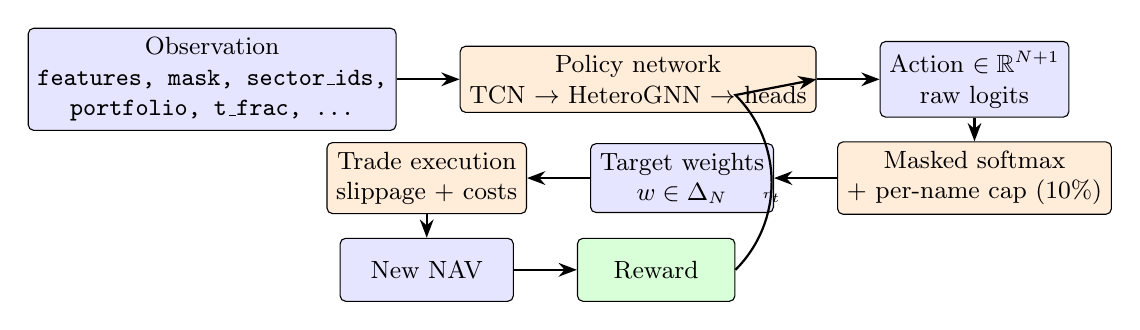
\begin{tikzpicture}[
  node distance=3mm and 8mm,
  box/.style={draw, rounded corners=2pt, minimum height=8mm, align=center, font=\small},
  data/.style={box, fill=blue!10, minimum width=22mm},
  proc/.style={box, fill=orange!15, minimum width=24mm},
  outp/.style={box, fill=green!15, minimum width=20mm},
  arrow/.style={-Stealth, thick}
]
\node[data] (obs) {Observation \\ \texttt{features, mask, sector\_ids,} \\ \texttt{portfolio, t\_frac, \ldots}};
\node[proc, right=of obs] (model) {Policy network \\ TCN $\to$ HeteroGNN $\to$ heads};
\node[data, right=of model] (act) {Action $\in \mathbb{R}^{N+1}$ \\ raw logits};
\node[proc, below=of act] (mask) {Masked softmax \\ + per-name cap (10\%)};
\node[data, left=of mask] (target) {Target weights \\ $w \in \Delta_N$};
\node[proc, left=of target] (exec) {Trade execution \\ slippage + costs};
\node[data, below=of exec] (nav) {New NAV};
\node[outp, right=of nav] (rwd) {Reward};
\draw[arrow] (obs) -- (model);
\draw[arrow] (model) -- (act);
\draw[arrow] (act) -- (mask);
\draw[arrow] (mask) -- (target);
\draw[arrow] (target) -- (exec);
\draw[arrow] (exec) -- (nav);
\draw[arrow] (nav) -- (rwd);
\draw[arrow] (rwd.east) to[bend right=45] node[below, font=\tiny]{$r_t$} ([yshift=-2mm]model.east -| rwd.east) -- (model.east);
\end{tikzpicture}
\caption{Per-step data flow inside \texttt{PanelTradingEnv}. The policy outputs raw
logits which are projected to the simplex with a per-name cap; trades are filled at
the open with ATR-scaled slippage; portfolio is marked-to-close; reward is computed
from the resulting log return.}
\label{fig:env-flow}
\end{figure}

\subsection{Observation Space}

The observation is a Gymnasium \texttt{Dict} with the following keys
(Table~\ref{tab:obs}). Note that the last three fields (\texttt{recent\_return\_1d},
\texttt{recent\_vol\_20d}, \texttt{nav\_log\_progress}) were added during the r6
critic-enrichment pass and are consumed only by the critic head.

\begin{table}[h]
\centering
\caption{Observation dictionary. $L = 60$ is the lookback, $N = 163$ is the universe
size, $F = 15$ is the feature count.}
\label{tab:obs}
\small
\begin{tabularx}{\textwidth}{l c X}
\toprule
\textbf{Key} & \textbf{Shape} & \textbf{Meaning} \\
\midrule
\texttt{features} & $(L, N, F)$ & Feature panel ending at $t-1$ \\
\texttt{mask} & $(N,)$ & \texttt{is\_tradeable} on day $t$ \\
\texttt{sector\_ids} & $(N,)$ & 1-indexed sector assignment (0 = unknown) \\
\texttt{portfolio} & $(N+1,)$ & Index 0 = cash weight; 1\ldots N = equity weights \\
\texttt{cash} & $()$ & Cash position in INR \\
\texttt{nav} & $()$ & Current net asset value \\
\texttt{t\_frac} & $()$ & Episode progress $\in [0, 1]$ \\
\texttt{recent\_return\_1d} & $()$ & Last day's portfolio log return \\
\texttt{recent\_vol\_20d} & $()$ & Std of last 20 daily log returns \\
\texttt{nav\_log\_progress} & $()$ & $\log(\text{NAV}_t / \text{NAV}_0)$ \\
\bottomrule
\end{tabularx}
\end{table}

\subsection{Action Space and the Masked Softmax Projection}

The action space is \texttt{Box}$(-10, 10, (N+1,))$ --- raw logits for cash and each
of the $N$ equity slots. The env applies a masked softmax with a per-name weight cap:

\begin{equation}
w_i = \begin{cases}
\frac{e^{\ell_i}}{\sum_{j \in \mathcal{V}} e^{\ell_j}}, & i \in \mathcal{V} \\
0, & i \notin \mathcal{V}
\end{cases}
\quad\text{where } \mathcal{V} = \{0\} \cup \{j : 1 \le j \le N, \text{mask}_j = 1\}
\end{equation}

Cash (slot 0) is always in $\mathcal{V}$. After the softmax, equity slots that
exceed the per-name cap $w_{\max} = 0.10$ are clipped, and the excess is
redistributed proportionally to all uncapped slots (cash and uncapped equities)
in a fixed-point iteration. Cash is never capped.

\subsection{Reward Functions}

Three reward functions are implemented (\texttt{src/trader/env/reward.py}):

\begin{description}[leftmargin=*]
\item[\texttt{LogReturn}] (current default) $r_t = \log(\text{NAV}_t / \text{NAV}_{t-1})$.
Direct, dense, aligned with CAGR maximization.

\item[\texttt{ExcessLogReturn}] (opt-in via \texttt{use\_excess\_returns} flag) the env
subtracts the cross-sectional mean of \texttt{log\_return\_1d} over tradeable stocks
before passing the value to the reward function:
\[ r_t = \log(\text{NAV}_t / \text{NAV}_{t-1}) - \overline{\rho}_t,\quad
   \overline{\rho}_t = \frac{1}{|\mathcal{V}_t|} \sum_{i \in \mathcal{V}_t} \log(p^{(i)}_t / p^{(i)}_{t-1}). \]

\item[\texttt{DifferentialSharpe}] (deprecated; retained for ablation) the
Moody--Saffell~\cite{moody2001} online gradient of the Sharpe ratio:
\[ \delta_t = \frac{B_{t-1} \Delta A_t - \tfrac{1}{2} A_{t-1} \Delta B_t}
                   {(B_{t-1} - A_{t-1}^2)^{3/2}}, \]
with $A, B$ EMAs of $r$ and $r^2$. We document in \S\ref{sec:debug} why this
is unsuitable for PPO with a value baseline.
\end{description}

A turnover penalty $-\lambda \cdot \tau_t$ is added on top, where $\tau_t$ is the L1
change in equity weights and $\lambda = 0.001$ by default.

\subsection{Cost Model}

\texttt{ZerodhaEquityDeliveryCostModel} implements the Indian equity delivery cost
schedule as of 2024 (Table~\ref{tab:costs}). Round-trip cost on a typical retail-size
trade is approximately 15--20 bps.

\begin{table}[h]
\centering
\caption{Zerodha equity delivery cost components. Rates apply to trade value in INR.}
\label{tab:costs}
\small
\begin{tabularx}{\textwidth}{l l X}
\toprule
\textbf{Component} & \textbf{Rate / Amount} & \textbf{Side} \\
\midrule
Brokerage & 0.03\%, capped at \textrm{Rs.}\,20/order & Both \\
STT & 0.10\% & Sell only \\
Exchange charge (NSE) & 0.00322\% & Both \\
GST & 18\% on (brokerage + exchange) & Both \\
SEBI charges & 0.0001\% & Both \\
Stamp duty & 0.015\% & Buy only \\
DP charge & \textrm{Rs.}\,15.93 per scrip per sell day & Sell only (per name) \\
\bottomrule
\end{tabularx}
\end{table}

\subsection{Slippage Model}

Fill price is the open of day $t$ adjusted by an ATR-scaled square-root impact:
\begin{equation}
\hat{p}_i = p^{\text{open}}_i \cdot \left(1 + k \cdot \frac{\text{ATR}_i}{p^{\text{close}}_i}
            \cdot \sqrt{\frac{|\Delta q_i|}{\text{ADV20}_i}}
            \cdot \operatorname{sgn}(\Delta q_i) \right),\quad k = 0.1
\end{equation}
where $\Delta q_i$ is the change in shares of name $i$ and ADV20 is the 20-day
average dollar volume divided by close. This is a standard retail-scale impact
model; institutional sizes would require a richer non-linear formula.

\subsection{Episode Termination}

An episode ends when either:
\begin{itemize}
\item $t \ge \texttt{episode\_length}$ (truncated at 252 days, capped to fit shorter
val/test panels), or
\item $\text{NAV}_t < 0.10 \cdot \text{NAV}_0$ (terminated --- a 90\% drawdown
ruin trigger).
\end{itemize}

% ════════════════════════════════════════════════════════════════════════════
\section{Model Architecture}
% ════════════════════════════════════════════════════════════════════════════

The policy is a three-stage pipeline (Figure~\ref{fig:arch}):

\begin{enumerate}
\item \textbf{Per-ticker encoder} --- a Temporal Convolutional Network (TCN) that
collapses each ticker's 60-day feature window into a $d$-dimensional embedding.
\item \textbf{Heterogeneous graph attention network} (HeteroGNN) over stocks and
sectors that produces context-refined embeddings.
\item \textbf{Actor / critic heads} that consume the refined embeddings together
with portfolio state.
\end{enumerate}

\begin{figure}[h]
\centering
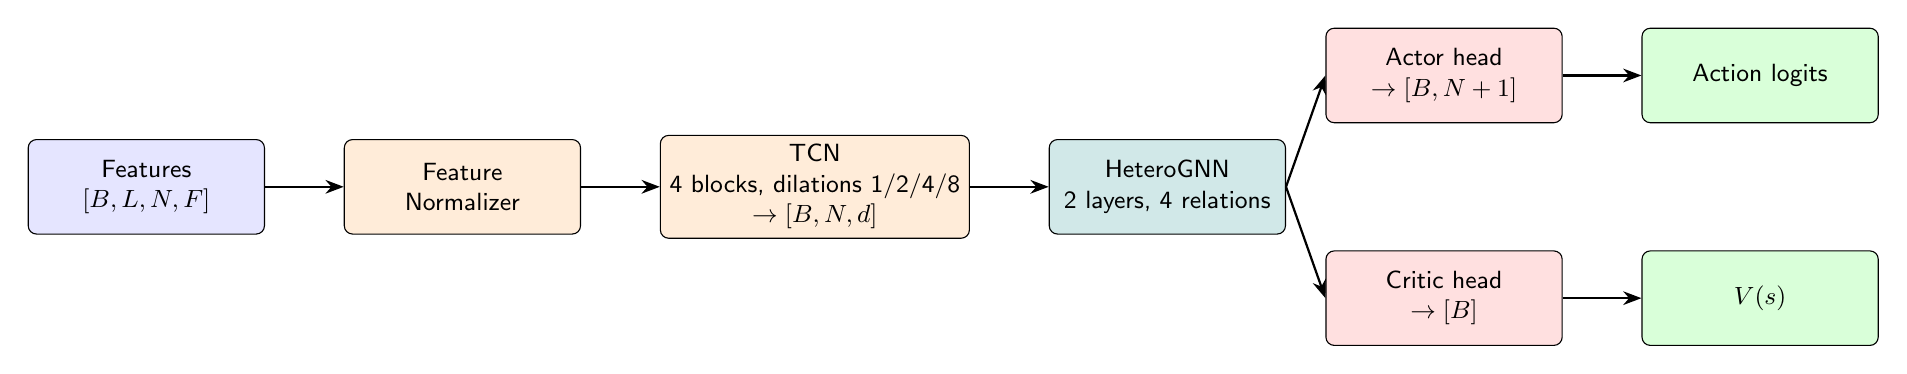
\begin{tikzpicture}[
  node distance=4mm and 10mm,
  blk/.style={draw, rounded corners=3pt, minimum height=12mm, minimum width=30mm,
              align=center, font=\small\sffamily},
  inp/.style={blk, fill=blue!10},
  enc/.style={blk, fill=orange!15},
  gnn/.style={blk, fill=teal!18},
  head/.style={blk, fill=red!12},
  outp/.style={blk, fill=green!15},
  ar/.style={-Stealth, thick}
]
\node[inp] (feat) {Features \\ $[B, L, N, F]$};
\node[enc, right=of feat] (norm) {Feature \\ Normalizer};
\node[enc, right=of norm] (tcn) {TCN \\ 4 blocks, dilations 1/2/4/8 \\ $\to [B, N, d]$};
\node[gnn, right=of tcn] (gnn) {HeteroGNN \\ 2 layers, 4 relations};
\node[head, above right=2mm and 5mm of gnn] (act) {Actor head \\ $\to [B, N+1]$};
\node[head, below right=2mm and 5mm of gnn] (crit) {Critic head \\ $\to [B]$};
\node[outp, right=of act] (logit) {Action logits};
\node[outp, right=of crit] (val) {$V(s)$};
\draw[ar] (feat) -- (norm);
\draw[ar] (norm) -- (tcn);
\draw[ar] (tcn) -- (gnn);
\draw[ar] (gnn.east) -- (act.west);
\draw[ar] (gnn.east) -- (crit.west);
\draw[ar] (act) -- (logit);
\draw[ar] (crit) -- (val);
\end{tikzpicture}
\caption{End-to-end policy architecture. The Feature Normalizer is a fixed
(non-trainable) buffer applied at the input of the encoder; see \S\ref{sec:debug}
for why it is essential.}
\label{fig:arch}
\end{figure}

\subsection{Feature Normalizer}

A fixed per-feature standardization layer applied at the encoder input:
\[ \tilde{x}_i = \frac{x_i - \mu_i}{\sigma_i},\quad
   \mu_i, \sigma_i \text{ computed from tradeable rows of the train panel.} \]

The mean and standard deviation are computed once at training start and stored as
non-trainable PyTorch buffers, so they save and load with the model. Validation
and test environments use the same statistics --- using their own would be a subtle
form of data leakage on the policy.

This component, while trivial in isolation, was the single largest accuracy fix
in the project. \S\ref{sec:debug} elaborates.

\subsection{TCN Encoder}

A four-block causal Temporal Convolutional Network~\cite{bai2018tcn} with
dilations $\{1, 2, 4, 8\}$. Each block contains two causal convolutions
(left-padded so the output length equals the input length), LayerNorm, GELU
activation, and dropout, with a residual connection. The receptive field after
four blocks of kernel size 3 is
\[ R = 1 + 2 \sum_{k=0}^{3} 2^k \cdot (3 - 1) = 31, \]
sufficient to capture intra-month structure in the 60-day window.

\begin{figure}[h]
\centering
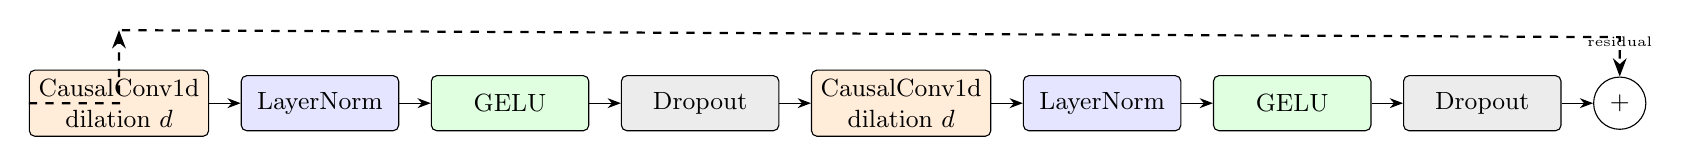
\begin{tikzpicture}[
  node distance=2mm,
  conv/.style={draw, rounded corners=2pt, minimum width=20mm, minimum height=7mm,
               fill=orange!15, align=center, font=\small},
  norm/.style={conv, fill=blue!10},
  act/.style={conv, fill=green!12},
  drop/.style={conv, fill=gray!15},
  ar/.style={-Stealth},
  res/.style={-Stealth, dashed, thick}
]
\node[conv] (c1) {CausalConv1d \\ \small dilation $d$};
\node[norm, right=4mm of c1] (n1) {LayerNorm};
\node[act, right=4mm of n1] (g1) {GELU};
\node[drop, right=4mm of g1] (d1) {Dropout};
\node[conv, right=4mm of d1] (c2) {CausalConv1d \\ \small dilation $d$};
\node[norm, right=4mm of c2] (n2) {LayerNorm};
\node[act, right=4mm of n2] (g2) {GELU};
\node[drop, right=4mm of g2] (d2) {Dropout};
\node[circle, draw, right=4mm of d2, minimum size=5mm, font=\small] (sum) {$+$};
\foreach \a/\b in {c1/n1, n1/g1, g1/d1, d1/c2, c2/n2, n2/g2, g2/d2, d2/sum} \draw[ar] (\a) -- (\b);
\draw[res] (c1.north) ++(0,0.5) coordinate (top);
\draw[res] (c1.west) -| (top) -- ($(sum.north) + (0, 0.5)$) -- (sum.north) node[midway, above, font=\tiny]{residual};
\end{tikzpicture}
\caption{Single TCN block. Four such blocks are stacked with dilations $\{1, 2, 4, 8\}$.}
\label{fig:tcn-block}
\end{figure}

The encoder consumes $[B, N, L, F]$ (after a permute from the env's
$[B, L, N, F]$ convention), reshapes to $[B \cdot N, F, L]$ for grouped per-ticker
processing, and emits $[B, N, d]$ by taking the last timestep of the final block:
$h_i = \text{TCN}(x_i)[:,:,-1] \in \mathbb{R}^d$. Weight sharing across tickers is
total --- there is one set of parameters for all $N$ stocks.

\subsection{Heterogeneous Graph Attention Network}

The graph has two node types and four relation types:

\begin{table}[h]
\centering
\caption{Node and edge types in the heterogeneous graph. $N = 163$, $S = 8$.}
\small
\begin{tabularx}{\textwidth}{l X}
\toprule
\textbf{Node} & \textbf{Description} \\
\midrule
\texttt{stock} & One node per equity, initialized from TCN output ($d$-dim) \\
\texttt{sector} & One node per sector, learnable embedding ($d$-dim) \\
\midrule
\textbf{Relation} & \textbf{Edges} \\
\midrule
\texttt{(stock, same\_sector, stock)} & All pairs $(i, j)$ with $\sigma(i) = \sigma(j)$, bidirectional \\
\texttt{(stock, in, sector)} & $(i, \sigma(i))$ for all tradeable $i$ \\
\texttt{(sector, contains, stock)} & Reverse of \texttt{in} \\
\texttt{(sector, relates\_to, sector)} & All pairs of distinct sectors, bidirectional \\
\bottomrule
\end{tabularx}
\end{table}

Each relation has its own \texttt{GATv2Conv}~\cite{brody2022gatv2} with $h = 2$
attention heads and \texttt{concat=False} (heads averaged so output dim equals input
dim regardless of head count). Two stacked HeteroConv layers with residual connections
and LayerNorm. \texttt{DropEdge}~\cite{rong2020dropedge} regularization (p=0.1)
randomly drops a fraction of edges per forward pass during training.

\subsubsection{A Concrete Six-Stock Example}

To make the graph structure tangible, consider a six-stock toy universe drawn from
three of the eight sectors:

\[
\text{Tickers} = (\text{RELIANCE},\ \text{ONGC},\ \text{HDFCBANK},\ \text{ICICIBANK},\ \text{INFY},\ \text{TCS})
\]

with sector vector $\sigma = (5, 5, 1, 1, 2, 2)$ (Oil/Power, Banking, IT). Suppose
all six are tradeable today, so $\text{mask} = (1,1,1,1,1,1)$.

The intra-sector adjacency matrix $A^{\text{intra}} \in \{0,1\}^{6 \times 6}$ is
\[
A^{\text{intra}} =
\begin{array}{r|cccccc}
       & \text{REL} & \text{ONGC} & \text{HDFC} & \text{ICICI} & \text{INFY} & \text{TCS} \\ \hline
\text{REL}   & 0 & 1 & 0 & 0 & 0 & 0 \\
\text{ONGC}  & 1 & 0 & 0 & 0 & 0 & 0 \\
\text{HDFC}  & 0 & 0 & 0 & 1 & 0 & 0 \\
\text{ICICI} & 0 & 0 & 1 & 0 & 0 & 0 \\
\text{INFY}  & 0 & 0 & 0 & 0 & 0 & 1 \\
\text{TCS}   & 0 & 0 & 0 & 0 & 1 & 0
\end{array}
\]

\texttt{GATv2Conv} adds self-loops for the \texttt{(stock, same\_sector, stock)} relation,
so the effective adjacency is $A^{\text{intra}} + I_6$.

The membership edge set is
$\{(0, 4), (1, 4), (2, 0), (3, 0), (4, 1), (5, 1)\}$
(0-indexed sectors), and the inter-sector relation is the complete bidirectional graph
on the three active sectors:
\[ \mathcal{E}^{\text{inter}} = \{ (0,1), (1,0), (0,4), (4,0), (1,4), (4,1) \}. \]

The full heterogeneous graph for this toy universe is illustrated in
Figure~\ref{fig:graph}.

\begin{figure}[h]
\centering
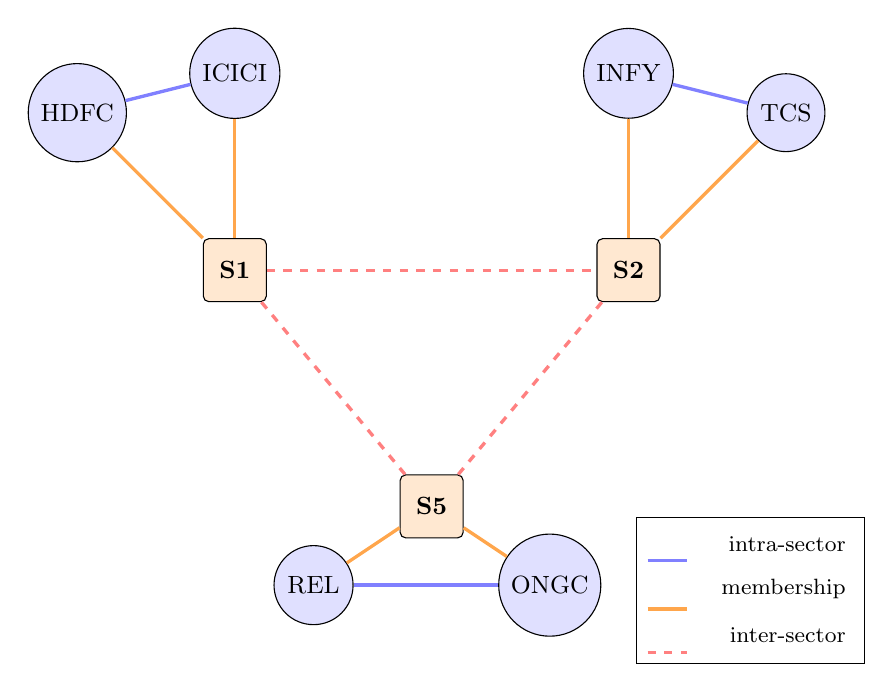
\begin{tikzpicture}[
  stockN/.style={draw, circle, minimum size=8mm, fill=blue!12, font=\small},
  sectorN/.style={draw, rectangle, rounded corners=2pt, minimum size=8mm,
                  fill=orange!18, font=\small\bfseries},
  intra/.style={very thick, blue!50, -},
  member/.style={very thick, orange!70, -},
  inter/.style={very thick, red!50, dashed, -}
]
% Sectors
\node[sectorN] (s1) at (0, 0) {S1};
\node[sectorN] (s2) at (5, 0) {S2};
\node[sectorN] (s5) at (2.5, -3) {S5};
% Banking sector stocks (top-left)
\node[stockN] (hdfc) at (-2, 2) {HDFC};
\node[stockN] (icici) at (0, 2.5) {ICICI};
% IT sector stocks (top-right)
\node[stockN] (infy) at (5, 2.5) {INFY};
\node[stockN] (tcs) at (7, 2) {TCS};
% Oil/Power sector stocks (bottom)
\node[stockN] (rel) at (1, -4) {REL};
\node[stockN] (ongc) at (4, -4) {ONGC};
% Intra-sector edges
\draw[intra] (hdfc) -- (icici);
\draw[intra] (infy) -- (tcs);
\draw[intra] (rel) -- (ongc);
% Membership edges
\draw[member] (hdfc) -- (s1);
\draw[member] (icici) -- (s1);
\draw[member] (infy) -- (s2);
\draw[member] (tcs) -- (s2);
\draw[member] (rel) -- (s5);
\draw[member] (ongc) -- (s5);
% Inter-sector edges
\draw[inter] (s1) -- (s2);
\draw[inter] (s1) -- (s5);
\draw[inter] (s2) -- (s5);
% Legend
\matrix [draw, fill=white, anchor=south east, column sep=3mm, row sep=1mm] at (8, -5) {
  \draw[intra] (0,0) -- (0.5,0); & \node[font=\footnotesize] {intra-sector}; \\
  \draw[member] (0,0) -- (0.5,0); & \node[font=\footnotesize] {membership}; \\
  \draw[inter] (0,0) -- (0.5,0); & \node[font=\footnotesize] {inter-sector}; \\
};
\end{tikzpicture}
\caption{Heterogeneous graph for the six-stock toy universe. Round nodes are stocks
(initialized from TCN output); rectangular nodes are sectors (learnable
embeddings). The full graph for the 163-stock universe has 163 stock nodes, 8
sector nodes, $\sum_s \binom{|s|}{2} \cdot 2 \approx 5{,}500$ intra-sector edges,
326 membership edges (163 in each direction), and 56 inter-sector edges.}
\label{fig:graph}
\end{figure}

\subsubsection{Batching and Masking}

The graph topology is identical for every batch element (same universe, same sector
assignments). The $B$ subgraphs are tiled into a single disconnected graph of $B \cdot N$
stock nodes and $B \cdot S$ sector nodes, so a single \texttt{HeteroConv} call processes
the entire batch.

Untradeable stocks have their input features zeroed before message passing
(\texttt{stock\_x = stock\_x * mask.unsqueeze(-1)}) so that stale or sentinel feature
values cannot leak into their neighbors' attention scores. They are also excluded
from the edge index in \texttt{build\_sector\_edges}.

\subsubsection{Ablation Variants}

Three configurations exist:
\begin{itemize}
\item \textbf{\texttt{mlp\_baseline}} --- no graph; encoder $\to$ mean-pool $\to$ heads.
The lower bound; a positive Sharpe here is a stretch goal.
\item \textbf{\texttt{gnn\_intra\_only}} --- only the
\texttt{(stock, same\_sector, stock)} relation; no sector nodes; no inter-sector edges.
The midpoint between MLP and full GNN.
\item \textbf{\texttt{gnn\_v1}} --- all four relations; sector nodes with learnable
embeddings; the full hetero-GAT.
\end{itemize}

\subsection{Actor and Critic Heads}

\subsubsection{Actor Head}

Per-ticker logits and a cash logit are produced by two parallel MLPs:
\begin{align}
p_i &= \text{MLP}_{\text{eq}}([z_i, w_i^{\text{eq}}]) \in \mathbb{R}, \quad i = 1 \ldots N \\
p_0 &= \text{MLP}_{\text{cash}}([\bar{z}, w^{\text{cash}}]) \in \mathbb{R}
\end{align}
where $z_i$ is the GNN output for stock $i$, $\bar{z}$ is its mean over $N$, and
$w_i$ are the current portfolio weights. The logit vector
$\ell = (p_0, p_1, \ldots, p_N)$ is the mean of a Gaussian policy with a learnable
per-dimension log-std parameter:
\[ a \sim \mathcal{N}(\ell, \operatorname{diag}(e^{2 \log\sigma})). \]
Initial $\log \sigma = -1$ (so $\sigma \approx 0.37$). The masked softmax / cap
projection is applied by the env, not the policy.

A critical detail (CleanRL convention~\cite{huang2022cleanrl}): the last linear layer
of each MLP is initialized with orthogonal weights at gain 0.01 and zero bias. This
keeps the initial logits at $\mathcal{O}(0.01)$, which after masked softmax gives a
near-uniform allocation at step 0 --- a stable starting point that does not blow up
the trust region during the first few PPO updates.

\subsubsection{Critic Head}

The critic takes a richer state summary:
\[ V(s) = \text{MLP}\left( [\bar{z},\ \overline{w}^{\text{eq}},\ \max w^{\text{eq}},\
   w^{\text{cash}},\ t_{\text{frac}},\ r_{1\text{d}},\ \sigma_{20\text{d}},\ \rho_{\text{NAV}},\
   e^{\text{sec}}] \right) \]
where the last block $e^{\text{sec}} \in \mathbb{R}^S$ is the per-sector portfolio
exposure, computed inside the critic head via a \texttt{scatter\_add} over
\texttt{sector\_ids} and the equity weights:
\[ e^{\text{sec}}_s = \sum_{\substack{i \\ \sigma(i) = s+1}} w_i^{\text{eq}}. \]

The added scalars ($r_{1\text{d}}$, $\sigma_{20\text{d}}$, $\rho_{\text{NAV}}$) come from
new observation keys backed by a 21-element rolling NAV history maintained in the env.
This enriched state lets the critic distinguish, e.g., ``+5\% at low vol'' from
``+5\% at high vol'' --- two states with identical NAV but very different forward
expectations.

The last linear layer of the critic uses orthogonal init at gain 1.0 (standard).

\subsection{Parameter Budget}

\begin{table}[h]
\centering
\caption{Approximate parameter count by component for the full \texttt{gnn\_v1}
configuration ($d = 64$, $h = 2$ heads, 2 GNN layers).}
\small
\begin{tabular}{l r}
\toprule
\textbf{Component} & \textbf{Parameters} \\
\midrule
TCN encoder (4 blocks) & $\sim$50k \\
HeteroGNN (2 layers, 4 relations) & $\sim$60k \\
Sector embedding ($S \times d$) & $\sim$0.5k \\
Actor head + log-std & $\sim$15k + 164 \\
Critic head & $\sim$15k \\
Feature Normalizer (buffer, non-trainable) & 30 \\
\midrule
\textbf{Total trainable} & $\sim$140k \\
\bottomrule
\end{tabular}
\end{table}

A trivial parameter count for the RTX 5090. The model size has \emph{deliberately}
not been scaled up: the architecture is sample-efficient for our setting and the
priority is to validate the pipeline before adding capacity.

% ════════════════════════════════════════════════════════════════════════════
\section{Reinforcement Learning Algorithm}
% ════════════════════════════════════════════════════════════════════════════

\subsection{Why PPO}

We use Proximal Policy Optimization~\cite{schulman2017ppo} for several reasons
specific to this task:

\begin{enumerate}[leftmargin=*]
\item \textbf{The action space is a constrained simplex.} A Gaussian over raw logits
followed by an in-environment masked softmax composes cleanly with PPO's clipped
likelihood ratio (the Jacobian of the projection does not enter the gradient).

\item \textbf{The state is large} ($\sim$600 KB per step). PPO's rollout buffer of
$\le$4096 samples is used once and discarded; an SAC-style replay buffer of
1M samples would require $\sim$600 GB.

\item \textbf{Off-policy data is contaminated by the agent's own portfolio history.}
Part of $s_t$ is the current portfolio, which is a consequence of past actions. PPO
is on-policy and avoids this.

\item \textbf{The environment is essentially deterministic.} Market data is fixed;
the only stochasticity is the random episode start. PPO's ``use samples once''
discipline is barely a tax when env steps are cheap.

\item \textbf{Training stability dominates peak performance.} PPO is famously hard
to break; SAC has more knobs (target entropy, automatic temperature, twin Q's) and
subtler failure modes. For a research project where any dial might be the cause of
failure, PPO's robustness is itself a feature.
\end{enumerate}

\subsection{The PPO Objective}

For each minibatch the loss is
\begin{equation}
\mathcal{L}(\theta) = \mathbb{E}_t \left[
\min(\rho_t A_t,\ \operatorname{clip}(\rho_t,\ 1-\epsilon,\ 1+\epsilon)\ A_t)
- c_v \cdot (V_\theta(s_t) - R_t)^2
+ c_e \cdot H[\pi_\theta(\cdot \mid s_t)]
\right]
\label{eq:ppo}
\end{equation}
where $\rho_t = \pi_\theta(a_t \mid s_t) / \pi_{\theta_{\text{old}}}(a_t \mid s_t)$
is the importance ratio, $A_t$ is the GAE estimator, $R_t = A_t + V_{\theta_{\text{old}}}(s_t)$
is the bootstrapped return target, $\epsilon = 0.2$ is the clip coefficient,
$c_v = 0.5$ is the value-loss weight, and $c_e = 0.001$ is the entropy bonus. The
value loss is additionally clipped:
\[ \mathcal{L}_v = \tfrac{1}{2} \max\left( (V_\theta - R)^2,\ (V_{\text{old}} +
\operatorname{clip}(V_\theta - V_{\text{old}}, -\epsilon, \epsilon) - R)^2 \right). \]

\subsection{Generalized Advantage Estimation}

GAE~\cite{schulman2016gae} is computed in reverse over the $T$-step rollout:
\begin{align}
\delta_t &= r_t + \gamma V(s_{t+1}) (1 - d_t) - V(s_t) \\
A_t &= \delta_t + \gamma \lambda (1 - d_t) A_{t+1}
\end{align}
with $\gamma = 0.995$ (matching the $\sim$200-day horizon) and $\lambda = 0.95$.

\subsection{Reward Normalization}

A Welford running standard deviation~\cite{welford1962} is maintained across the
entire training run; rewards are divided by it before GAE. The mean is
\emph{not} subtracted --- preserving sign matters for distinguishing good vs bad
trades. This keeps the gradient scale stable as the policy improves and reward
magnitudes change.

\subsection{Mixed-Precision Training}

Forward and backward passes run under \texttt{torch.autocast(dtype=torch.bfloat16)}
on CUDA. BF16's wider exponent range avoids the gradient scaling needed for FP16,
and BF16 values round-trip losslessly through FP32, so casting to numpy for env
interaction is safe. A subtle bug arose when only the update used BF16 while the
rollout did not (\S\ref{sec:debug}); the fix was to share a single \texttt{autocast}
context across both phases.

\subsection{Target-KL Early Stopping}

After each minibatch the approximate KL divergence
\[ \widehat{\text{KL}} = \mathbb{E}_t[(\rho_t - 1) - \log \rho_t] \]
is checked; if its mean over an epoch exceeds 0.02, the remaining epochs are
skipped. This protects against runaway updates when the policy and the rollout
distribution have drifted apart.

\subsection{Algorithm Summary}

\begin{algorithm}[h]
\caption{PPO training loop (one update iteration)}
\label{alg:ppo}
\begin{algorithmic}[1]
\State $\textbf{model.eval}()$ \Comment{disable DropEdge / dropout for deterministic log-probs}
\State $\textbf{amp\_ctx} \gets \texttt{autocast}(\text{BF16, enabled} = \text{cuda})$
\State $\text{rollout buffers} \gets \emptyset$
\State \textbf{with} \texttt{torch.no\_grad(), amp\_ctx:}
\For{$t = 1 \ldots T$}
  \State Sample action $a_t$ from $\pi_{\theta_{\text{old}}}(\cdot \mid s_t)$
  \State Step env: $(s_{t+1}, r_t, d_t) \gets \text{env}(s_t, a_t)$
  \State Append $(s_t, a_t, \log \pi(a_t), V(s_t), r_t, d_t)$ to buffer
\EndFor
\State Bootstrap $V(s_T)$ for last state
\If{normalize\_rewards}
  \State Update $\widehat{\sigma}_r$; $r_t \gets r_t / \widehat{\sigma}_r$
\EndIf
\State Compute $A_t, R_t$ via GAE
\State Anneal LR: $\eta \gets \eta_0 \cdot (1 - \text{update}/\text{n\_updates})$
\For{$\text{epoch} = 1 \ldots E$}
  \State Shuffle and split into $M$ minibatches
  \For{each minibatch}
    \State \textbf{with} \texttt{amp\_ctx:} compute $\log \pi_\theta(a)$, $H[\pi_\theta]$, $V_\theta(s)$
    \State Normalize advantages: $A \gets (A - \bar{A}) / \sigma_A$
    \State Compute $\mathcal{L}$ per Eq.~\eqref{eq:ppo}
    \State Backprop, clip grad norm, Adam step
  \EndFor
  \State \textbf{if} $\overline{\text{KL}} > 0.02$ \textbf{break} \Comment{target-KL early stop}
\EndFor
\end{algorithmic}
\end{algorithm}

% ════════════════════════════════════════════════════════════════════════════
\section{A Step-by-Step Walkthrough}
\label{sec:walkthrough}
% ════════════════════════════════════════════════════════════════════════════

To make the system concrete, we trace one training step end to end on the toy
six-stock universe from \S4.3.1, with $L = 60$, $F = 15$, $d = 64$.

\textbf{Step 0: Observation.} The env returns
\begin{itemize}
\item \texttt{features}: a $60 \times 6 \times 15$ tensor; each $(\ell, n, f)$ entry
is the feature $f$ for stock $n$ on day $t - 60 + \ell$.
\item \texttt{mask}: $(1, 1, 1, 1, 1, 1)$.
\item \texttt{sector\_ids}: $(5, 5, 1, 1, 2, 2)$.
\item \texttt{portfolio}: $(1, 0, 0, 0, 0, 0, 0)$ at episode start --- 100\% cash.
\item \texttt{t\_frac}: $0.0$.
\item \texttt{recent\_return\_1d}, \texttt{recent\_vol\_20d}, \texttt{nav\_log\_progress}: $0.0$ each.
\end{itemize}

\textbf{Step 1: Feature normalization.} Each of the 15 feature channels is
standardized using buffers $\mu_f, \sigma_f$ computed at training start. For example,
\texttt{dollar\_volume\_20} for RELIANCE on this day might be 8.5e9; the normalizer
maps this to $(8.5\text{e9} - 1.29\text{e9}) / 2.44\text{e9} = 2.96$, putting it on
the same numerical scale as \texttt{log\_return\_1d}.

\textbf{Step 2: TCN encoding.} The $60 \times 15$ window for each stock is
processed through 4 dilated causal conv blocks. The final timestep output is
a $d = 64$ vector $h_i$ per stock --- a learned summary of the past quarter.

\textbf{Step 3: Hetero graph attention.}
\begin{enumerate}
\item Stock embeddings $h \in \mathbb{R}^{6 \times 64}$ are zeroed where mask is 0
(here, none).
\item Sector embeddings are looked up: $E^{\text{sec}} \in \mathbb{R}^{8 \times 64}$.
\item Edges are constructed (Figure~\ref{fig:graph}) and DropEdge is applied
(eval mode in rollout, so a no-op). The edge dictionary is tiled across the batch.
\item One \texttt{HeteroConv} call processes all four relations:
\begin{align}
h_i^{(1)} &= \text{LayerNorm}\Big( \text{GELU}\big(
  \text{HeteroAgg}(h, E^{\text{sec}}, \mathcal{E})_i
\big) + h_i \Big) \\
E_s^{\text{sec}, (1)} &= \text{LayerNorm}\Big( \text{GELU}\big(
  \cdots
\big) + E_s^{\text{sec}} \Big)
\end{align}
\item A second layer is applied analogously, producing the final stock representation
$z \in \mathbb{R}^{6 \times 64}$.
\end{enumerate}

\textbf{Step 4: Actor head.} For each stock $i$,
$p_i = \text{MLP}_{\text{eq}}([z_i, w_i^{\text{eq}}])$.
At init (small-init weights), all $p_i \approx 0$ and similarly $p_0 \approx 0$.
The Gaussian policy samples
\[ a \sim \mathcal{N}(\ell, \sigma^2 I),\quad \ell \approx \mathbf{0},\ \sigma \approx 0.37, \]
yielding raw logits roughly in $[-0.7, +0.7]$.

\textbf{Step 5: Critic head.} A scalar value
\[ V(s) = \text{MLP}([\bar{z},\ \text{summary scalars (7)},\ \text{sector exposures (8)}]) \]
is computed. At init it is also near zero.

\textbf{Step 6: Action projection in env.} The masked softmax with cap is applied:
$w = \texttt{masked\_softmax}(a, \text{mask}, w_{\max}=0.10)$.
At init with $\sigma = 0.37$, sample logits give $w$ roughly uniform around
$1/(N+1) \approx 0.14$ on the toy universe (or $\approx 0.006$ per slot on the full
163-stock universe before the cap kicks in).

\textbf{Step 7: Trade execution.} Target shares are computed at the open with floor
rounding; slippage is applied; costs are deducted; the new position is marked to
close. NAV update gives $\log r_t = \log(\text{NAV}_t / \text{NAV}_{t-1})$.

\textbf{Step 8: Reward.} With the default \texttt{LogReturn} reward and turnover
penalty $\lambda = 0.001$,
\[ r_t = \log r_t - \lambda \tau_t. \]

\textbf{Step 9: Buffer.} The full $(s_t, a_t, \log \pi(a_t), V(s_t), r_t, d_t)$
tuple is appended to the rollout buffer. After $T = 256$ such steps across each of
$E = 16$ envs, the PPO update consumes the resulting $4096$-sample batch.

% ════════════════════════════════════════════════════════════════════════════
\section{The Debugging Journey}
\label{sec:debug}
% ════════════════════════════════════════════════════════════════════════════

This section is included not for completeness but because the debugging arc
\emph{is} the result. Each bug masqueraded as a different one; fixing the wrong one
first would have produced no improvement and led us to abandon a working
architecture.

\subsection{Run-by-Run Status}

\begin{table}[h]
\centering
\caption{Training run history. ``r5'' refers to the fifth restart of the GNN runs
prior to identifying the BF16/FP32 precision bug; ``r6'' is the current run with all
known fixes. Final figures are training-set Sharpe over the last 10 episodes.}
\scriptsize
\begin{tabularx}{\textwidth}{l X r r X}
\toprule
\textbf{Run} & \textbf{Code state} & \textbf{Train Sharpe} & \textbf{Val Sharpe} & \textbf{Notes} \\
\midrule
r1--r4 & DSR + train()-mode rollout & diverged & --- & GNN clip\_frac=1, KL=36--161 \\
r5 MLP & DSR + eval() & $-1.33$ & $-2.09$ & Stable, uniform policy \\
r5 GNN\_v1 & DSR + BF16/FP32 fix & $-1.39$ & --- & Killed pre-completion \\
r5 GNN\_intra & DSR + BF16/FP32 fix & $-1.89$ & --- & Killed pre-completion \\
\midrule
r6 MLP & LogReturn + feat-norm + crit-enrich + actor-init & $-1.12$ & $-1.66$ & Better than r5 \\
r6 GNN\_v1 & + above & $-2.36$ & --- & At 32\% --- concerning \\
r6 GNN\_intra & + above & $\mathbf{+0.031}$ & --- & At 44\% --- first positive! \\
\bottomrule
\end{tabularx}
\end{table}

\subsection{Bug 1: Stochastic Operations During Rollout}

\textbf{Symptom.} GNN runs diverged with \texttt{clip\_frac = 1.000} and
\texttt{approx\_kl = 36--161} from the very first update. MLP runs were unaffected.

\textbf{Diagnosis.} \texttt{torch.no\_grad()} disables gradient tracking but does
\emph{not} disable dropout or any other stochastic operation. With the model in
\texttt{train()} mode during rollout, both \texttt{DropEdge} (random edge removal,
$p = 0.1$) and \texttt{GATv2Conv}'s attention dropout fire. The rollout's
$\log \pi_{\theta_{\text{old}}}(a)$ was computed under one random graph topology; the
update's $\log \pi_\theta(a)$ was computed under a \emph{different} topology. The
importance ratio $\exp(\log \pi_\theta - \log \pi_{\theta_{\text{old}}})$ was measuring
random topology change, not weight change.

The MLP was less affected only because TCN dropout has smaller functional impact
than two layers of graph attention plus DropEdge.

\textbf{Fix.} Call \texttt{self.model.eval()} before the rollout and restore
\texttt{self.model.train()} only at the end of the training loop. \emph{Forgetting
this is a silent killer for any RL policy with stochastic operations in the
forward path.}

\subsection{Bug 2: BF16 / FP32 Precision Mismatch}

\textbf{Symptom.} Even after Bug 1 was fixed, GNN runs showed
\texttt{clip\_frac = 0.978} on the very first PPO update --- before any gradient
step had been applied. Identical pre-update weights were producing different
log-probs in rollout vs update.

\textbf{Diagnosis.} The rollout was running in plain FP32 (no autocast); the
update was wrapped in BF16 \texttt{autocast}. BF16 has 7 mantissa bits versus
FP32's 23, giving roughly $0.8\%$ relative error per matmul. Over two
\texttt{GATv2Conv} layers (each with multiple matmuls per attention head), the
error compounds to several percent, which is enough to shift logits by
$O(0.1)$ and explode the KL.

\textbf{Severity correlated with depth.} GNN\_v1 (4 edge types, more matmuls)
showed KL = 161; GNN\_intra (1 edge type) showed KL = 50.8; MLP (no graph)
showed clip\_frac = 0.065 --- mild but present.

\textbf{Fix.} Create the \texttt{autocast} context \emph{before} the rollout and
use it in both \texttt{with torch.no\_grad(), amp\_ctx:} and \texttt{with amp\_ctx:}
update blocks. Cast model outputs to FP32 before \texttt{.cpu().numpy()} (BF16 is
not a numpy dtype).

\subsection{Bug 3: \texttt{DifferentialSharpe} Reward Has Zero Expected Value}

\textbf{Symptom.} After Bugs 1 and 2 were fixed, the MLP trained stably to
Sharpe $-1.33$ over 8M steps. The agent did not catastrophically fail, but it
also did not learn to trade. The policy converged to a high-entropy, near-uniform
allocation. CAGR was $-16.6\%$ in a market where the equal-weight baseline returns
$+16.4\%$ (a 33-percentage-point gap).

\textbf{Diagnosis.} The DSR formula
\[ \delta_t = \frac{B_{t-1} (r_t - A_{t-1}) - \tfrac{1}{2} A_{t-1} (r_t^2 - B_{t-1})}{(B - A^2)^{3/2}} \]
at steady state simplifies to $\delta_t \approx C \cdot (r_t - \mu_t)$ where $\mu_t$
is the running EMA mean of returns. Its expected value is therefore \emph{zero},
regardless of whether $\mu_t$ is positive (good portfolio) or negative (bad
portfolio). The PPO value head learned $V(s) \approx 0$ for all $s$; advantages
became pure noise; the only remaining gradient was from the entropy bonus
($c_e = 0.001$), which slowly randomized the policy.

DSR was designed for direct policy gradient (REINFORCE) where its zero-mean
property is fine because there is no value baseline. With a critic in PPO it
fails.

\textbf{Fix.} Switch to plain $r_t = \log(\text{NAV}_t / \text{NAV}_{t-1})$
(\texttt{LogReturn}). Bonus bug found in passing: the YAML key \texttt{reward:
differential\_sharpe} was \emph{never read} by \texttt{train.py} --- the env
always used the default \texttt{DifferentialSharpe} regardless of config. We wired
up a \texttt{\_REWARD\_MAP} in \texttt{train.py}.

\subsection{Bug 4: Feature Scale Catastrophe}

\textbf{Symptom.} Even after switching to LogReturn, the MLP made only modest
gains and the agent still allocated near-randomly. The model was trained but
shouldn't have been --- feature scales differed by eleven orders of magnitude.

\textbf{Diagnosis.} See the std column of Table~\ref{tab:features}. Without
input normalization, the TCN's first conv layer applies
$\mathbf{W} x \in \mathbb{R}^{C \times L}$ with $\mathbf{W}$ at Xavier scale
$\mathcal{O}(1/\sqrt{F})$. The pre-LayerNorm output for
\texttt{dollar\_volume\_20} is $\sim 10^9 \cdot 0.25 = 2.5 \times 10^8$; for
\texttt{log\_return\_1d} it is $\sim 10^{-2} \cdot 0.25 = 2.5 \times 10^{-3}$.
After LayerNorm the dollar-volume signal dominates the entire normalized output
and the small-scale signals (returns, RSI, momentum, vol) are reduced to numerical
noise. The model has effectively been allocating based on a noisy ranking of
20-day dollar volume.

\textbf{Fix.} A fixed \texttt{FeatureNormalizer} layer at the encoder input,
applying $(x - \mu) / \sigma$ where $\mu, \sigma$ are computed from the
\emph{tradeable} rows of the train panel. Stats are saved to
\texttt{data/panels/train.feature\_stats.json} alongside the panel SHA256.

This fix alone moved MLP train Sharpe from $-1.33$ to $-1.12$ and enabled
GNN\_intra to reach the first positive Sharpe of the project.

\subsection{Bug 5: Environment Was the Wall-Clock Bottleneck}

\textbf{Symptom.} 8M steps took roughly 12 hours on the RTX 5090 at $\sim$185
SPS across 16 envs --- around 11 SPS per env. GPU utilization was 15--20\%.

\textbf{Diagnosis.} \texttt{PanelTradingEnv.\_build\_obs()} contained a
double Python for-loop over $(\text{features}, \text{tickers})$ with dict
lookups: $60 \times 163 \times 15 = 146{,}700$ Python operations per step.
\texttt{\_price\_at()}, \texttt{\_mask\_at()}, \texttt{\_sector\_ids\_at()} each
did 163 dict lookups per call. The cost calculation in \texttt{step()} was
another per-ticker Python loop over the 163-name universe. The GPU was
starved waiting for the env.

\textbf{Fix.} At env construction:
\begin{itemize}
\item Pre-stack features to a single $[T, N, F]$ NumPy array.
\item Pre-stack each price/metadata column to $[T, N]$.
\item Pre-stack the tradeable mask to $[T, N]$ bool.
\end{itemize}
Then \texttt{\_build\_obs()} is a single slice operation; \texttt{\_price\_at()}
is a single index; the cost loop is replaced by a vectorized
\texttt{cost\_vec()} method on the cost model that uses pure NumPy.

\textbf{Measured impact.} Single-env step rate jumped from $\sim$11 SPS to
$\sim$12{,}000 SPS --- roughly 1{,}000$\times$ speedup on the env alone. End-to-end
training is now GPU-bound; r6 MLP achieved 254 SPS (37\% above the r5 baseline
of 185 SPS) and r6 GNN\_intra is at 142 SPS.

\subsection{Architectural Hardening (Beyond Bugs)}

Two additional improvements were applied in the same r6 pass:

\textbf{Critic enrichment.} The critic head was given access to per-sector
exposure (8 dims via \texttt{scatter\_add}) and three new portfolio scalars
(recent return, recent vol, NAV log progress). Lower critic variance
$\Rightarrow$ lower advantage variance $\Rightarrow$ more stable PPO updates.

\textbf{Small-init actor.} Both actor MLPs' final linear layers are initialized
with orthogonal weights at gain 0.01 (CleanRL convention). The pre-softmax logits
at step 0 are bounded by $\sim$0.018, giving a near-uniform allocation. This is the
standard cure for early-training KL spikes in PPO.

% ════════════════════════════════════════════════════════════════════════════
\section{Empirical Results}
% ════════════════════════════════════════════════════════════════════════════

\subsection{Baselines}

The baseline reference is \texttt{equal\_weight\_rebalanced} on the train panel:
\textbf{Sharpe = 1.04, CAGR = 16.4\%, vol = 15.7\%}. This is the bar the RL agent
must beat on \emph{validation} for M5/M6 acceptance.

\subsection{r6 Results In Progress}

\begin{table}[h]
\centering
\caption{Current r6 metrics as of April 26, 2026, mid-run. The MLP completed
training; the two GNN runs are in progress.}
\small
\begin{tabularx}{\textwidth}{l r r r r r r}
\toprule
\textbf{Run} & \textbf{Update} & \textbf{Train Sharpe} & \textbf{Val Sharpe} & \textbf{CAGR} & \textbf{Clip frac} & \textbf{SPS} \\
\midrule
mlp\_baseline & 1953/1953 & $-1.12$ & $-1.66$ & $-13.8\%$ & 0.004 & 254 \\
gnn\_v1 & 630/1953 & $-2.36$ & --- & $-30.7\%$ & 0.298 & 104 \\
gnn\_intra\_only & 860/1953 & $\mathbf{+0.031}$ & --- & $\mathbf{+7.3\%}$ & 0.324 & 142 \\
\bottomrule
\end{tabularx}
\end{table}

The most encouraging signal is \texttt{rew\_std} = 0.010 across all three runs ---
exactly the LogReturn scale (daily log return std on a diversified Indian equity
portfolio is $\sim 1\%$). With the previous DSR reward this metric was 4--7. The
fact that all three runs show $\text{clip\_frac} \in [0.30, 0.32]$ is a textbook
healthy band.

\subsection{Why GNN\_v1 Underperforms GNN\_intra}

A surprising and currently un-explained result: the simpler intra-only graph
materially outperforms the full hetero-GNN through the first $\sim$30\% of training.
A working hypothesis (to be confirmed in r7): PyTorch's default
\texttt{nn.Embedding} initialization is $\mathcal{N}(0, 1)$, but the LayerNorm-ed
TCN output has unit norm. The sector embeddings are therefore $\sim 8\times$ larger
than the stock embeddings entering the GNN, and via the
\texttt{(sector, contains, stock)} relation they dominate the message passing for
hundreds of updates. The intra-only variant has no sector nodes and is immune.

The fix (one line) is queued for r7:
\begin{lstlisting}
nn.init.normal_(self.sector_emb.weight, mean=0.0, std=0.1)
\end{lstlisting}

% ════════════════════════════════════════════════════════════════════════════
\section{Hyperparameter Reference}
% ════════════════════════════════════════════════════════════════════════════

\subsection{PPO Hyperparameters}

\begin{table}[h]
\centering
\small
\caption{PPO hyperparameter cheat-sheet --- what each knob does and the empirical
range that produced healthy training in r6.}
\begin{tabularx}{\textwidth}{l c X}
\toprule
\textbf{Param} & \textbf{Value} & \textbf{Effect} \\
\midrule
\texttt{learning\_rate} & 3e-4 (MLP) / 5e-5 (GNN) & GNN attention layers have larger gradient norms; smaller LR prevents trust-region exits \\
\texttt{clip\_coef} ($\epsilon$) & 0.2 & PPO ratio clipping threshold; 0.2 is canonical \\
\texttt{ent\_coef} ($c_e$) & 0.001 & Lower than PPO defaults (0.01) --- at 0.01 entropy dominated the gradient signal in this task \\
\texttt{vf\_coef} ($c_v$) & 0.5 & Standard \\
\texttt{max\_grad\_norm} & 0.5 (MLP) / 0.2 (GNN) & GNN grad norms are larger; tighter clipping required \\
\texttt{gamma} ($\gamma$) & 0.995 & $\sim$200-day effective horizon (vs 252-day episode) \\
\texttt{gae\_lambda} ($\lambda$) & 0.95 & Standard bias/variance tradeoff \\
\texttt{n\_steps} & 256 & Rollout length per env \\
\texttt{n\_envs} & 16 & SyncVectorEnv worker count \\
\texttt{n\_minibatches} & 32 & 32, not 64 --- 64 caused excessive sequential drift in r4 \\
\texttt{n\_epochs} & 4 & Standard; combined with target\_kl early stopping \\
\texttt{target\_kl} & 0.02 & Threshold for early-stopping the epoch loop \\
\texttt{normalize\_advantage} & true & Per-minibatch zero-mean unit-std \\
\texttt{normalize\_rewards} & true & Welford running std, mean NOT subtracted \\
\texttt{anneal\_lr} & true & Linear decay to 0 at final update \\
\bottomrule
\end{tabularx}
\end{table}

\subsection{Model Hyperparameters}

\begin{table}[h]
\centering
\small
\caption{Model hyperparameters and the components they affect.}
\begin{tabularx}{\textwidth}{l c X}
\toprule
\textbf{Param} & \textbf{Value} & \textbf{Affects} \\
\midrule
\texttt{embed\_dim} ($d$) & 64 & TCN output, GNN node dim, head input \\
\texttt{kernel\_size} & 3 & TCN receptive field $\propto$ kernel \\
\texttt{num\_channels} & [64, 64, 64, 64] & TCN depth and width \\
\texttt{dropout} (TCN) & 0.1 & Generalization; only active in train() mode \\
\texttt{num\_layers} (GNN) & 2 & Message-passing depth; $k$-hop neighborhood \\
\texttt{num\_heads} (GAT) & 2 & Attention diversity \\
\texttt{dropout} (GAT) & 0.1 & Attention regularization \\
\texttt{drop\_edge\_prob} & 0.1 & DropEdge regularization; only active in train() \\
\texttt{relations} & all / intra\_only & Ablation control \\
\texttt{num\_sectors} & 8 & Critic exposure dim, sector embedding count \\
\texttt{head\_hidden} & 64 & Width of actor / critic MLPs \\
\texttt{log\_std\_init} & $-1$ ($\sigma \approx 0.37$) & Initial Gaussian policy std \\
\bottomrule
\end{tabularx}
\end{table}

\subsection{Environment Hyperparameters}

\begin{table}[h]
\centering
\small
\caption{Environment hyperparameters.}
\begin{tabularx}{\textwidth}{l c X}
\toprule
\textbf{Param} & \textbf{Value} & \textbf{Affects} \\
\midrule
\texttt{lookback\_days} & 60 & Feature window length $L$ \\
\texttt{episode\_length} & 252 & Trading days per episode (auto-clamped on shorter panels) \\
\texttt{initial\_cash} & \textrm{Rs.}\,1{,}000{,}000 & Realistic retail account size for NSE \\
\texttt{max\_weight\_per\_name} & 0.10 & Diversification floor; min $\sim$10 names if fully invested \\
\texttt{turnover\_penalty} & 0.001 & L1 weight-change penalty in reward \\
\texttt{reward} & log\_return & vs differential\_sharpe / excess\_log\_return \\
\texttt{use\_excess\_returns} & false & Subtract benchmark before reward (opt-in) \\
\bottomrule
\end{tabularx}
\end{table}

% ════════════════════════════════════════════════════════════════════════════
\section{Future Work}
% ════════════════════════════════════════════════════════════════════════════

\subsection{r7: Pre-staged Improvements}

The following changes are already implemented and gated as opt-in (so they did
not perturb the in-flight r6 runs):

\begin{enumerate}
\item \textbf{Sector embedding init at $\mathcal{N}(0, 0.1)$.}
Active on fresh runs only.
\item \textbf{\texttt{ExcessLogReturn} reward + \texttt{use\_excess\_returns} env flag.}
Subtracts the cross-sectional mean log return from the portfolio log return before
reward computation, giving the agent a direct incentive to beat the universe
average rather than just earn positive returns.
\item \textbf{Lower \texttt{ent\_coef} to 1e-4.}
End-of-r6 diagnostics show $\sigma$ drifting from 0.37 to $\sim$0.65 over training.
A 10$\times$ smaller entropy bonus will tighten the policy in late training without
hurting early exploration.
\item \textbf{Per-batch tradeable mask in GNN edge construction.}
Currently \texttt{mask[0]} is reused for every batch element. Untradeable stocks are
correctly zeroed in features but still appear as graph nodes with messaging
contributions. Deferred until results indicate it matters.
\end{enumerate}

\subsection{M7: Walk-Forward Training}

\texttt{src/trader/training/walk\_forward.py} (not yet implemented) will run
\textbf{4 windows} of (24-month train, 1-month purge, 6-month val, 6-month test)
sliding through the full panel, with \textbf{5 seeds} per window. A paired
bootstrap CI of RL agent vs \texttt{equal\_weight} on each window is the
acceptance test. A shuffled-ticker-label sanity check is wired behind a flag to
detect spurious signal exploitation.

\subsection{M8--M10: Paper Broker, Live Stub, End-to-End Report}

The remaining three milestones are scoped:
\begin{itemize}
\item \textbf{M8}: Paper broker backed by Postgres ledger; T+1 cash settlement;
golden-file integration test (fixed seed $\to$ fixed fills).
\item \textbf{M9}: Zerodha Kite Connect adapter stub (interface only,
\texttt{NotImplementedError} bodies).
\item \textbf{M10}: \texttt{full\_report.py} producing a single PDF with equity
curves, drawdown, per-sector allocation over time, GNN attention heatmap, and
paired bootstrap significance tables.
\end{itemize}

\subsection{Beyond M10: Possible Extensions}

Only after M10 (a complete walk-forward baseline that beats \texttt{equal\_weight})
is in hand are the following worth considering:
\begin{itemize}
\item Sentiment embeddings (offline; per-(ticker, week) static representations).
\item Hierarchical two-level policy: weekly sector allocation (slow) + daily
within-sector picks (fast).
\item Intraday data and a new env variant (5-minute bars).
\item Soft Actor-Critic ablation (after PPO has been proven sufficient).
\item Live adapter (separate stream with its own risk review).
\end{itemize}

% ════════════════════════════════════════════════════════════════════════════
\section{Lessons Learned}
% ════════════════════════════════════════════════════════════════════════════

A few practical conclusions earned the hard way during M5--M6:

\begin{enumerate}[leftmargin=*]
\item \textbf{Algorithm choice rarely fixes a broken environment, reward, or
feature pipeline.} We considered switching to SAC mid-debug; doing so would have
hidden Bug 4 (feature normalization) for weeks and confounded the diagnosis with
SAC's own tuning subtleties. The discipline of fixing the environment first paid
off.

\item \textbf{The stochastic-rollout bug is universal for graph or
high-dropout policies.} \texttt{torch.no\_grad()} is not a substitute for
\texttt{model.eval()}. Any RL pipeline that uses DropEdge, attention dropout, or
batch-norm-style stochastic operations should call eval() during rollout.

\item \textbf{Reward functions for PPO must have non-zero expected value at
optimum.} The Differential Sharpe is mathematically elegant but unsuited for an
algorithm with a value baseline. Reward design and algorithm design are coupled.

\item \textbf{Feature scale standardization is the cheapest large-effect fix
in deep RL.} A single \texttt{FeatureNormalizer} buffer moved a $-1.33$ Sharpe
agent into the regime where actual learning is possible.

\item \textbf{Profile the env before assuming the GPU is the bottleneck.} A
1{,}000$\times$ env speedup turned a CPU-bound 12-hour run into a GPU-bound
3--5-hour run with no model changes.

\item \textbf{Logs are not enough; instrument early.} \texttt{clip\_frac},
\texttt{approx\_kl}, and \texttt{rew\_std} caught bugs that final-Sharpe alone
would have hidden behind seed variance.
\end{enumerate}

% ════════════════════════════════════════════════════════════════════════════
\begin{thebibliography}{99}
% ════════════════════════════════════════════════════════════════════════════

\bibitem{schulman2017ppo}
J.~Schulman, F.~Wolski, P.~Dhariwal, A.~Radford, O.~Klimov.
\newblock \textit{Proximal Policy Optimization Algorithms}.
\newblock arXiv:1707.06347, 2017.

\bibitem{schulman2016gae}
J.~Schulman, P.~Moritz, S.~Levine, M.~Jordan, P.~Abbeel.
\newblock \textit{High-Dimensional Continuous Control Using Generalized Advantage
Estimation}.
\newblock ICLR, 2016.

\bibitem{bai2018tcn}
S.~Bai, J.~Z.~Kolter, V.~Koltun.
\newblock \textit{An Empirical Evaluation of Generic Convolutional and Recurrent
Networks for Sequence Modeling}.
\newblock arXiv:1803.01271, 2018.

\bibitem{velickovic2018gat}
P.~Veli\v{c}kovi\'c, G.~Cucurull, A.~Casanova, A.~Romero, P.~Li\`o, Y.~Bengio.
\newblock \textit{Graph Attention Networks}.
\newblock ICLR, 2018.

\bibitem{brody2022gatv2}
S.~Brody, U.~Alon, E.~Yahav.
\newblock \textit{How Attentive are Graph Attention Networks?}
\newblock ICLR, 2022.

\bibitem{schlichtkrull2018rgcn}
M.~Schlichtkrull, T.~N.~Kipf, P.~Bloem, R.~van~den~Berg, I.~Titov, M.~Welling.
\newblock \textit{Modeling Relational Data with Graph Convolutional Networks}.
\newblock ESWC, 2018.

\bibitem{rong2020dropedge}
Y.~Rong, W.~Huang, T.~Xu, J.~Huang.
\newblock \textit{DropEdge: Towards Deep Graph Convolutional Networks on Node
Classification}.
\newblock ICLR, 2020.

\bibitem{moody2001}
J.~Moody, M.~Saffell.
\newblock \textit{Learning to Trade via Direct Reinforcement}.
\newblock IEEE Transactions on Neural Networks, 12(4), 2001.

\bibitem{huang2022cleanrl}
S.~Huang, R.~F.~J.~Dossa, C.~Ye, J.~Braga, D.~Chakraborty, K.~Mehta, J.~G.~Ara\'ujo.
\newblock \textit{CleanRL: High-quality Single-file Implementations of Deep
Reinforcement Learning Algorithms}.
\newblock JMLR, 2022.

\bibitem{welford1962}
B.~P.~Welford.
\newblock \textit{Note on a Method for Calculating Corrected Sums of Squares and
Products}.
\newblock Technometrics, 4(3), 1962.

\bibitem{haarnoja2018sac}
T.~Haarnoja, A.~Zhou, P.~Abbeel, S.~Levine.
\newblock \textit{Soft Actor-Critic: Off-Policy Maximum Entropy Deep
Reinforcement Learning with a Stochastic Actor}.
\newblock ICML, 2018.

\bibitem{liu2022finrl}
X.-Y.~Liu et al.
\newblock \textit{FinRL: Deep Reinforcement Learning Framework to Automate
Trading in Quantitative Finance}.
\newblock ACM ICAIF, 2022.

\bibitem{moody1998}
J.~Moody, L.~Wu, Y.~Liao, M.~Saffell.
\newblock \textit{Performance Functions and Reinforcement Learning for Trading
Systems and Portfolios}.
\newblock Journal of Forecasting, 17, 1998.

\end{thebibliography}

\end{document}
